% Insert in the relevant Methods subsection; compile from overleaf/SWBAM/.
\begin{figure*}[!t]
    \centering
    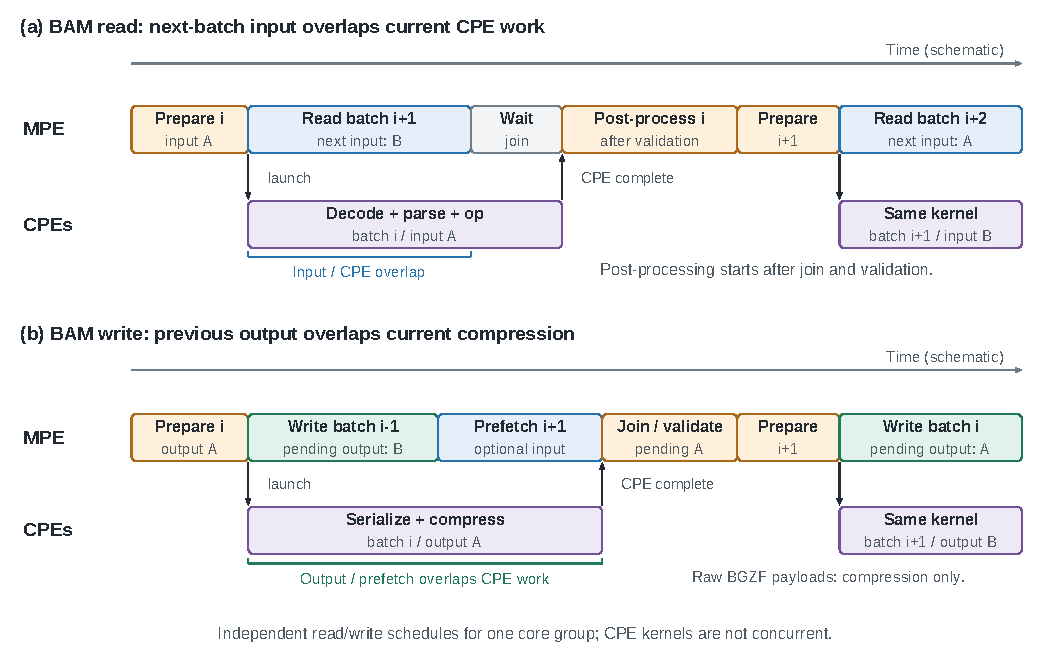
\includegraphics[width=\textwidth]{../figs/swbam_batch_overlap.pdf}
    \caption{Batch-level MPE--CPE overlap within one core group.
    (a) With read-side input overlap enabled, the MPE reads the next batch into
    the alternate input buffer while the CPEs process the current batch;
    batch post-processing follows CPE completion and validation.
    (b) With write-side output overlap enabled, the MPE emits a previously
    compressed batch while the CPEs process the current batch. Optional
    next-input prefetch is shown. Bars are schematic, not measured durations;
    the two panels are separate schedules, not concurrent read/write kernels.}
    \label{fig:swbam_batch_overlap}
\end{figure*}
